\section{Analysis}
\subsection{Speedup}
The execution times measured are shown in table~\ref{tab:exectimes}. The \emph{Gaussian blurring} and the overall execution times were both measured separately. For the \emph{Gaussian\_smoothing} code, the speedup is for the \emph{slower} of the two:
% $\frac{baseline}{\max(dsp,neon)}$ 
${baseline}/{\max(dsp,neon)}$ 
The total speedup is simply computed as 
%$\frac{baseline}{optimized}$. 
${baseline}/{optimized}$.
A speedup of a factor of over two is achieved, meaning that the new execution time is more than two times faster than the baseline implementation.

\emph{TODO, maybe talk about amdall's law here to justify the speedup of 2 versus 4?}

\begin{table*}
\centering
\begin{tabular}{l | r r r r | r r r}
        & \multicolumn{4}{|c|}{Gaussian}                & \multicolumn{3}{|c}{Total}                \\
Image   & Baseline  & DSP   & NEON          & Speedup   & Baseline  & Optimized         & Speedup   \\
\hline
Square  & 30605     & 5768  & 6745          & 4.537     & 42291     & 20325             & 2.081     \\
Tiger   & 77270     & 15137 & 15625         & 4.945     & 108520    & 49896             & 2.175     \\
Klomp   & 160455    & 29449 & 29510         & 5.437     & 228814    & 101349            & 2.257     \\
\end{tabular}
\caption{The execution times measured in $\mu$s}
\label{tab:exectimes}
\end{table*}

\begin{table*}
\centering
\begin{tabular}{l | r r r | r r r r r}
        & \multicolumn{3}{|c|}{Baseline}    & \multicolumn{5}{|c}{Optimized}                        \\
Image   & Gaussian  & Total     & Rest      & Gaussian  & Total     & Rest  & Overhead  & Ratio     \\
\hline
Square  & 30605     & 42291     & 11686     & 6745      & 20325     & 13580 & 1894      & 0.093     \\
Tiger   & 77270     & 108520    & 31250     & 15625     & 49896     & 34271 & 3021      & 0.061     \\
Klomp   & 160455    & 228814    & 68359     & 29510     & 101349    & 71839 & 3480      & 0.034     \\
\end{tabular}
\caption{Calculating the overhead as a fraction, all times in $\mu$s}
\label{tab:overhead}
\end{table*}


\begin{figure*}
    \centering
    \begin{subfigure}[b]{0.3\textwidth}
            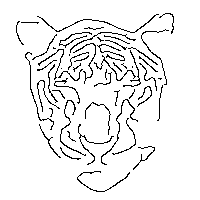
\includegraphics[width=\textwidth]{tiger_baseline}
            \caption{The baseline result}
            \label{fig:er_tiger_baseline}
    \end{subfigure}
    \begin{subfigure}[b]{0.3\textwidth}
            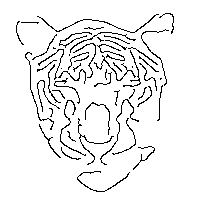
\includegraphics[width=\textwidth]{tiger_out}
            \caption{The optimized result}
            \label{fig:er_tiger_out}
    \end{subfigure}
    \begin{subfigure}[b]{0.3\textwidth}
            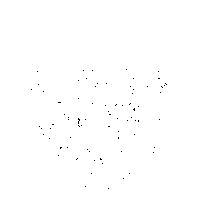
\includegraphics[width=\textwidth]{tiger_diff}
            \caption{The output of Algorithm~\ref{alg:imgdiff}}
            \label{fig:er_tiger_diff}
    \end{subfigure}
    \caption{Using the error visualization on an image of a tiger}
    \label{fig:imgdiff}
\end{figure*}


An interesting followup question is the amount of overhead we have introduced in the rest of the application. This overhead is in the form of for example allocating the shared memory pool and taking care of communication and synchronization. To calculate this, we subtracted for both the baseline and optimized versions the guassian execution times from the total execution times to obtain the rest execution times. We then subtract the baseline rest from the optimized rest to obtain the overhead time. This overhead time is divided by the total optimized execution time to calculate the overhead factor.


\subsection{Error Analysis}
Some slight inaccuracies (for example using a fixed-point representation instead of floating point in the DSP) have been introduced due to several changes in the algorithm; hence, errors (deviations from the reference implementation) are to be expected. 
Large errors are obvious to the eye, but this might be less obvious if the errors are only small. In this chapter we will detect and quantify these errors, to ensure that our implementation can still be considered correct.

\subsubsection{Error Visualization}
Visualizing our errors is a fairly straightforward process. Because both images are constructed out of pixels with a grayscale value from 0 (black) to 255 (white), we can construct a new image by taking the difference between each pixel as a new pixel value. Note that this would give us a mapping where black indicates no difference, and brighter pixels indicating the difference. The inverse has more visual pop-out, so we subtract the difference from 255 to obtain our final pixel value. The implementation is described in Algorithm \ref{alg:imgdiff}. The result of this algorithm and a further comparison between the baseline and our implementation can be seen in figure~\ref{fig:imgdiff}.

An interesting observation is that all the errors are in the lower area of the image, which is indeed the part that has been blurred by the DSP in a fixed point representation\footnote{This image has been produced with the load balancing of 35\% and 65\% for NEON and DSP respectively}.

\begin{algorithm}[t]
    \caption{Constructing a image with the differences between two images}\label{alg:imgdiff}
    \begin{algorithmic}[1]
        \Procedure{DiffImage}{$A[N],B[N]$}
        \State $C[N]\gets 0$
        \For{$i\gets 0, n-1$}
           \State $C[i]\gets 255 - |A[i] - B[i]|$
        \EndFor
        \State \textbf{return} $C$
        \EndProcedure
    \end{algorithmic}
\end{algorithm}

\subsubsection{Error quantification}



\begin{table}
    \centering
    \begin{tabular}{l | l l l l}
    Image   & Reference MSE & Optimized MSE & Difference    & Ratio     \\
    \hline
    Square  & 10643.08      & 10906.21      & 263.12        & 0.0247    \\
    Tiger   & 46683.48      & 46678.21      &   5.27        & 0.0001    \\
    Klomp   & 20535.52      & 20509.07      &  26.45        & 0.0013
    \end{tabular}
    \caption{The calculated mean squared error}
    \label{tab:mse}
\end{table}

In the visualization we can clearly spot some differences, but further quantification would be useful. For this, we decided to use the \emph{Mean Squared Error(MSE)}, as defined in (\ref{eq:mse}). This is an error-estimator giving a quantification of the error rate. Since this number on its own has little meaning, it was decided to calculate the MSE rate of the baseline implementation and the optimized versions, both with respect to the original image and calculate the ratio between the difference and the reference error rate, to give an error estimation. The results are given in table~\ref{tab:mse}. We find the final error ratio to be acceptable.

\begin{equation}
    MSE = \frac{1}{n} \sum_{i=0}^{n-1} (A[i] - B[i])^{2}
    \label{eq:mse}
\end{equation}